\documentclass[journal]{IEEEtran}
\hyphenation{op-tical net-works semi-conduc-tor}
\usepackage[utf8]{inputenc}
\usepackage{graphicx}
\usepackage[justification=centering]{caption} %caption居中
%\usepackage[sorting=none]{biblatex}
%\addbibresource{reference.bib}
\usepackage{booktabs} % 表格
\usepackage{float}  %引入float宏包
\usepackage{bm} % 加黑
\usepackage{xcolor}% 字体颜色
\usepackage[table]{xcolor}

\usepackage{amsmath}%数学公式
\usepackage[numbers,sort&compress]{natbib}
%\usepackage{siunitx} % For proper alignment of numbers
\usepackage[section]{placeins}
\usepackage{caption} % For table captions

% 图片依赖的路径
\graphicspath{{chapter and images}}
\begin{document}
\title{HMIF:An Efficient Infrared and RGB Image Fusion Network Based on HVI}
\author{Yi~Li, Huajun~Wang}

\markboth{}
{Shell \MakeLowercase{\textit{et al.}}: Bare Demo of IEEEtran.cls for Journals}
\maketitle

\begin{abstract}
Infrared and visible image fusion combines the thermal target information from infrared images with the textural details from visible images, significantly enhancing scene perception. However, differences in image acquisition between infrared and RGB sensors introduce key challenges. Firstly, RGB images are susceptible to luminance noise under low-light conditions, degrading fusion quality. Secondly, existing methods often simply superimpose multi-sensor information, neglecting the distinct characteristics of different modalities, which leads to loss of critical information or redundancy. To address these limitations, we propose the HVI Adaptive Brightness Enhancement module to improve fusion stability and accuracy under low-light conditions. Furthermore, based on the existing EMMA framework, we integrate the HVI module with mainstream fusion modules to construct an asymmetric dual-branch fusion architecture. Experimental results demonstrate that the proposed method achieves superior subjective visual quality and objective evaluation metrics in infrared-visible image fusion tasks, effectively enhancing fusion performance in complex scenes.

\end{abstract}

\begin{IEEEkeywords}
Image fusion, unsupervised learning, 
\end{IEEEkeywords}
\IEEEpeerreviewmaketitle
\section{Introduction}
Visible and Infrared Image Fusion (VIF) synthesizes images captured by different sensors, typically infrared and visible spectrum images, into a single composite representation. The core objective is to integrate complementary and redundant information from these source images, generating a fused result richer in information than any individual input. This enhanced imagery significantly benefits downstream processing tasks across diverse fields including digital photography, remote sensing, agriculture, medicine, and biometrics \cite{ma2019infrared}.
Visible images exhibit high spatial resolution and rich textural detail, closely aligning with human visual perception. However, their quality is highly vulnerable to occlusion, illumination variations, and adverse weather conditions. Infrared imaging, based on thermal radiation capture, offers superior penetration capabilities (through media like smoke or mist) and effectively distinguishes materials through emissivity differences. Infrared images typically suffer from lower spatial resolution, edge blurring due to thermal diffusion effects, and prominent non-uniformity noise and temporal noise.

Consequently, a primary challenge in VIF stems from the fundamentally distinct physical properties captured by each modality: thermal radiation versus light reflection. This divergence places their respective features on separate manifolds \cite{luo2023infrared}. Naïve linear fusion strategies, such as weighted averaging, frequently induce feature conflict. For example, a high-temperature region appearing bright in the infrared image might correspond to a low-brightness region in the visible image.
Existing VIF approaches fall primarily into traditional methods and deep learning-based techniques. Traditional methods typically follow a three-stage process: feature extraction (e.g., texture from visible images and salient thermal targets from infrared images) using specific transforms like multi-scale decomposition; application of predefined fusion rules within the transformed domain; and reconstruction of the fused image via the inverse transform \cite{luo2023infrared}. The reliance on manually designed steps and parameters limits their robustness and ability to produce high-quality fusion results across diverse real-world scenarios \cite{lin2022review}.

Driven by significant advancements in deep learning for image processing, substantial research focuses on leveraging these techniques for VIF \cite{luo2023infrared}. Based on network architecture, deep VIF methods are categorized into CNN-based, Autoencoder-based, Generative Adversarial Network-based, Transformer-based, and hybrid approaches. CNN-based methods (\cite{Hou2020VIFNet}) effectively capture local features but struggle with long-range dependencies. Autoencoder-based methods, such as DenseFuse \cite{Hui2019DenseFuse}, pre-train an encoder-decoder structure using infrared and visible image pairs. Hand-crafted rules (e.g., addition, L1-norm) then merge the extracted features before the decoder reconstructs the fused image. While yielding reasonable results, dependence on manual fusion rules often leads to suboptimal performance. Generative Adversarial Network-based methods (e.g., DDcGAN \cite{Jiayi2020DDcGAN}) employ discriminators to guide generators towards producing fused images matching source distributions. Nevertheless, these methods suffer from interpretability issues, control difficulties, training instability, and potential texture distortion. Transformer-based approaches (e.g., SePT \cite{yang2024semantic}) leverage self-attention for effective long-range modeling, albeit often with high computational complexity. Hybrid architectures represent the current mainstream, aiming to combine advantages. For instance, CMFuse \cite{Zhao2024CMFuse} focuses on optimizing cross-modal interactions, while EMMA \cite{zhao2024equivariant} utilizes outputs from existing fusion algorithms to learn sensor distribution properties for training guidance. Hybrid methods still demonstrate limitations in complex scenarios involving uneven illumination and strong noise.

Despite progress in integrating key complementary information from infrared and visible images, significant challenges persist: (1) Visible images suffer severe detail loss in underexposed/overexposed regions under extreme illumination variations, which existing algorithms inadequately address; (2) Predominant frameworks typically apply symmetric feature extraction paths \cite{lin2022review}, hindering integration with adaptive enhancement strategies for visible inputs;

To address these limitations, this paper presents three core contributions: 
\begin{itemize}
    \item \textbf{HVI Adaptive Brightness Enhancement Strategy:} We propose an HVI adaptive brightness enhancement strategy. This strategy effectively enhances the stability of the fusion process and the robustness of the results under low-light and uneven illumination conditions.
    \item \textbf{Asymmetric Dual-Branch Fusion Framework:} We construct an asymmetric dual-branch fusion framework. This framework, termed the Asymmetric Dual-Branch Fusion Framework , integrates the HVI module with a mainstream fusion module. It employs a two-stage fusion approach to separate the enhanced visible image and the original infrared image.
    \item \textbf{Experimental Results:} Experimental results demonstrate that our fusion model significantly improves the color richness of visible images, exhibits stronger detail preservation capabilities, mitigates noise interference, and markedly enhances the visibility of target objects within scenes.
\end{itemize}


\section{METHODOLOGY}
\label{sec:method}
\subsection{HVI Transformation}
\label{ssec:hvi}
Low-Light Image Enhancement (LLIE) aims to improve visual quality under poor illumination conditions, with core challenges involving effective noise suppression and color distortion mitigation. Current methodologies predominantly process images in standard RGB space \cite{yan2025hvi}. However, natural scene imagery exhibits high sensitivity to brightness fluctuations due to illumination variations, occlusions, and shadows. The fundamental limitation of RGB representation lies in the tight coupling of luminance and chrominance information: brightness variations induce correlated changes across all three channels (R, G, B), preventing independent manipulation of lightness and color.

To address this limitation, conversion to HSV color space is frequently employed. This perceptual model decouples color attributes into three orthogonal components:
\begin{align}
\text{Hue (H)} &:\ \text{dominant wavelength} \\
\text{Saturation (S)} &:\ \text{color purity} \\
\text{Value (V)} &:\ \text{brightness intensity}
\end{align}
The separation facilitates improved color denoising and luminance restoration. RGB-to-HSV conversion proceeds as follows. Given $R, G, B \in [0, 255]$, first normalize components:
\begin{equation}
R' = \frac{R}{255}, \quad G' = \frac{G}{255}, \quad B' = \frac{B}{255}
\end{equation}
Compute extrema and differential:
\begin{align}
C_{\text{max}} &= \max(R', G', B') \\
C_{\text{min}} &= \min(R', G', B') \\
\Delta &= C_{\text{max}} - C_{\text{min}}
\end{align}
Hue ($H$) is then derived:
\begin{equation}
H = 
\begin{cases}
0^\circ & \Delta = 0 \\
60^\circ \times \left( \frac{G' - B'}{\Delta} \mod 6 \right) & C_{\text{max}} = R' \\
60^\circ \times \left( \frac{B' - R'}{\Delta} + 2 \right) & C_{\text{max}} = G' \\
60^\circ \times \left( \frac{R' - G'}{\Delta} + 4 \right) & C_{\text{max}} = B'
\end{cases}
\end{equation}
Saturation ($S$) and Value ($V$) follow:
\begin{equation}
S = 
\begin{cases}
0 & C_{\text{max}} = 0 \\
\Delta / C_{\text{max}} & \text{otherwise}
\end{cases}, \quad
V = C_{\text{max}}
\end{equation}

Despite advantages in luminance-chrominance separation, HSV introduces noticeable red-band artifacts and dark-region noise during enhancement, particularly degrading perceptual quality in saturated reds and shadows. To overcome these artifacts, we introduce the HVI color space \cite{yan2025hvi}, which decomposes sRGB images into:
\begin{align}
\text{Intensity map } (I_{\text{max}}) &:\ \text{scene illuminance} \\
\text{HV color map } (\hat{H},\hat{V}) &:\ \text{chromatic structure}
\end{align}
where $I_{\text{max}}$ is computed per-pixel as:
\begin{equation}
I_{\text{max}}(x) = \max\limits_{c \in \{R,G,B\}} I_c(x)
\end{equation}

HVI eliminates hue discontinuities through polar encoding:
\begin{equation}
H = \cos\left(\frac{\pi h}{3}\right), \quad 
V = \sin\left(\frac{\pi h}{3}\right)
\end{equation}
where $h \in H$ and $v \in V$ represent orthogonal components. This formulation ensures continuous representation across the hue spectrum (notably eliminating red-region artifacts) while minimizing Euclidean distances between perceptually similar colors.

Noise amplification in low-light regions is suppressed via adaptive intensity compression:
\begin{equation}
C_k(x) = \sqrt[k]{\sin\left(\frac{\pi I_{\text{max}}(x)}{2}\right) + \varepsilon}
\end{equation}
where the learnable parameter $k$ controls compression strength. This function implements radial mapping, with small $C_k$ values concentrating low-intensity regions. The transformed components are then obtained by:
\begin{equation}
\hat{H} = C_k \odot S \odot H, \quad \hat{V} =  C_k \odot S \odot V
\end{equation}
where $\odot$ denotes the Hadamard product. Final HVI representation concatenates $\hat{H}$, $\hat{V}$, and $I_{\text{max}}$.

In multispectral fusion frameworks, visible images transformed to HVI yield HV maps $(\hat{H},\hat{V})$ and $I_{\text{max}}$, while infrared images provide complementary intensity data. These components are channel-concatenated and fed into enhancement modules, leveraging HVI's artifact suppression and signal fidelity preservation properties.




\subsection{Enhance HVI Fusion Module}
\label{ssec:fusion}
The enhancement fusion module comprises an HV feature branch and an intensity (I) feature branch. Initial feature extraction is performed using $3\times3$ convolutions. Subsequently, a U-Net architecture-based fusion network (Fig. \ref{fig:pipeline}) integrates multimodal features. This network embeds multiple Cross-Attention Blocks (CABs) and incorporates skip connections between its encoder and decoder.

The cross-attention mechanism establishes bidirectional guidance between the two branches. Features extracted by the intensity (I) branch dynamically modulate feature responses in the HV branch via attention weights, enabling brightness-adaptive noise suppression (enhanced denoising in low-light regions while preserving original color in bright regions). Crucially, the optimized HV features simultaneously feed back structural and textural color information to the I branch, constraining the enhancement process to mitigate halo artifacts. This design is grounded in the physical observation that noise intensity varies inversely with illumination intensity, necessitating region-specific processing.

The decoder outputs two enhanced feature maps: the enhanced HV features ($\hat{HV_e}$) and the enhanced intensity features ($\hat{I_e}$). These features are concatenated along the channel dimension and fed into the Post-HVI Inverse Transform (PHVIT) module to reconstruct the enhanced sRGB output image.

The PHVIT module reverses the transformation. It decomposes $\hat{HV_e}$ into its orthogonal components $\hat{H_e}$ and $\hat{V_e}$ using learned parameters $C_k$ and $\epsilon$, computing intermediate variables $\hat{h}$ and $\hat{v}$:
\begin{equation}
\begin{aligned}
\hat{h}=\frac{\hat{H_e}}{C_k+\epsilon} \\
\hat{v}=\frac{\hat{V_e}}{C_k+\epsilon}
\end{aligned}
\end{equation}
Subsequently, $\hat{h}$, $\hat{v}$, and $\hat{I_e}$ are transformed back to the standard HSV color space:
\begin{equation}
\begin{aligned}
H_{new} &= \arctan(\frac{{\hat{v}}'}{\hat{h}'}) \mod 1  \\
S_{new} &= \alpha_s \sqrt{{(\hat{v}}')^{2} + {(\hat{h}}')^{2}} \\
V_{new} &= \alpha_{i} \hat{I_e}
\end{aligned}
\end{equation}
where $\alpha_s$ and $\alpha_{i}$ are learnable linear parameters scaling saturation and intensity weights, respectively. Finally, the components $H_{new}$, $S_{new}$, and $V_{new}$ are converted from the HSV color space to the standard sRGB color space, yielding the enhanced output image.

\begin{figure*}[!t]
    \centering
    \includegraphics[width=1.0\textwidth]{chapter and images/enhance_fusion.png}
    \caption{Overview of the Enhanced Fusion Network Architecture. (a) HVI Color Transformation Module (HVIT): Transforms visible light into the HVI color space, obtaining its HV channels and intensity map, alongside the infrared image's intensity map. (b) Enhanced Fusion Network: Employs a dual-branch UNet architecture as its core, integrating six lightweight Cross-Attention Block (CAB) modules. (c) Perceptual Inverse HVI Transformation (PHVIT): Converts the enhanced HVI representation back into the RGB format, producing the final enhanced fused image.}
    \label{fig:pipeline}
\end{figure*}

\subsection{Enhanced EMMA Framework with Equivariant Imaging Prior}
\label{ssec:maf}

\begin{figure*}[!t]
    \centering
    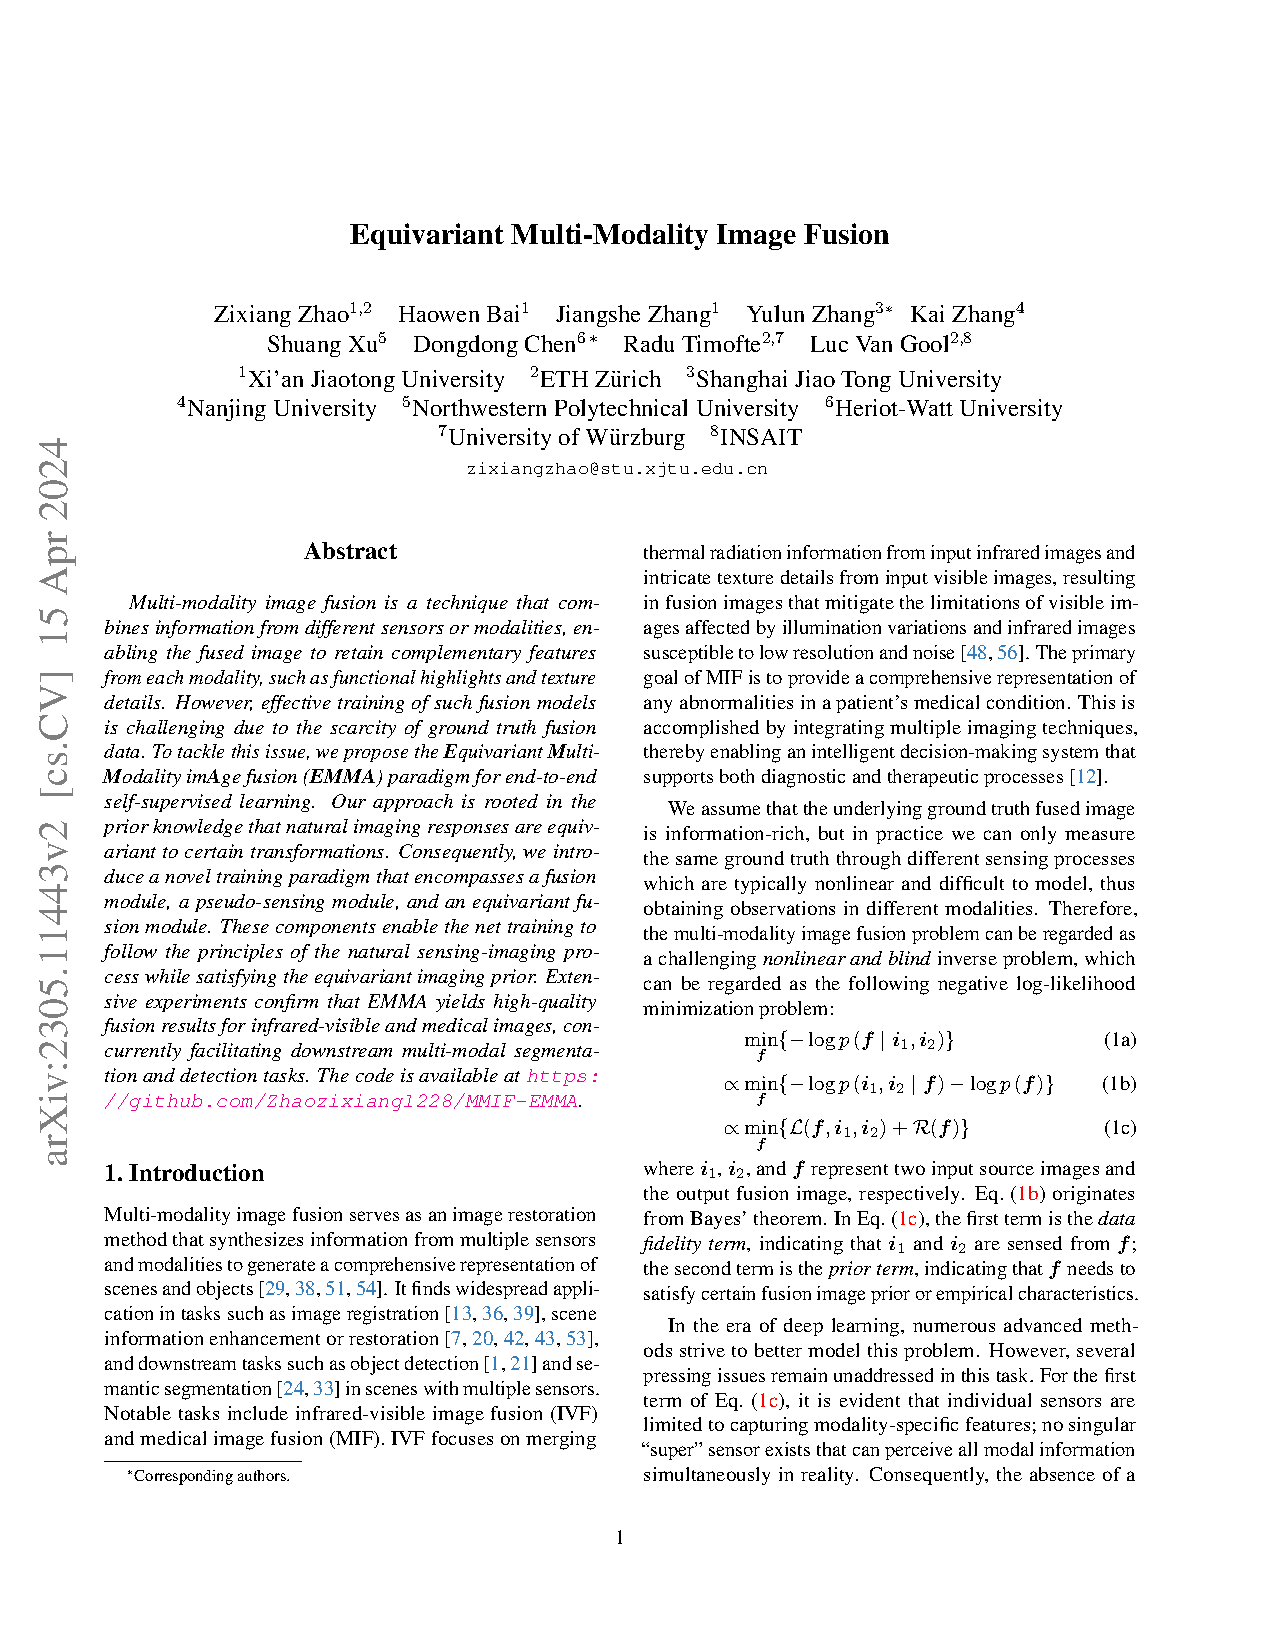
\includegraphics[width=1.0\textwidth]{chapter and images/EMMA.png}
    \caption{改进EMMA自监督融合网络架构概述(a)HVI Fusion:Enhanced HVI Fusion Network(b)等变模块:用于数据增强(c)伪传感器模块:普通UNet网络,经过训练后freeze,只负责推理。}
    \label{fig:EMMA}
\end{figure*}

To effectively leverage multi-modal fusion information, we propose the Enhanced Multi-modal self-supervised fusion frAmework (EMMA), which integrates an equivariant imaging prior. EMMA adapts the inherent pattern of its loss function by simulating the sensing imaging process based on natural imaging principles. The core workflow of EMMA is illustrated in Figure \ref{fig:EMMA}.

During training, the original infrared ($i$) and visible ($v$) images are first input into the HVI Fusion network (Fig. \ref{fig:EMMA}(a)). This network acts as the fusion backbone, extracting and integrating information from both modalities to produce a preliminary fused feature map $f$.

Subsequently, $f$ is processed by the Equivariant Module (Fig. \ref{fig:EMMA}(b)), which applies predefined geometric transformations (e.g., rotation, translation, reflection) to generate a transformed fused image $f_t$. This step is grounded in the Equivariant Imaging Prior, which posits that the representation of a fusion result should exhibit corresponding consistency under these transformations. The augmentation enhances model robustness and generalization in the absence of direct supervision.

The transformed image $f_t$ is then fed into two independent, pre-trained pseudo-sensor modules: an infrared pseudo-sensor module $A_i$ and a visible pseudo-sensor module $A_v$. Both modules utilize a standard U-Net architecture. These modules are trained with pseudo ground truth generated from state-of-the-art fusion algorithms to learn the mapping from the fused image back to the original source images. During EMMA's main training phase, the weights of these pseudo-sensor modules remain frozen; they function solely as "inverse decoders" performing forward inference to assess whether $f_t$ retains sufficient information for reconstructing the source images. Consequently, $A_i$ infers a pseudo-infrared image $\hat{i}_t$ and $A_v$ infers a pseudo-visible image $\hat{v}_t$.

Finally, the pseudo-infrared $\hat{i}_t$ and pseudo-visible $\hat{v}_t$ images are cycled back as input into the same HVI Fusion network, producing the final fused output $\hat{f_t}$.

\subsection{Loss Function}
Our framework incorporates loss functions for infrared images, visible images, and the final fused output. The total loss \(L_{\text{total}}\) is computed as a weighted combination of these three components:
\begin{equation}\label{equ}
    \begin{aligned}
    L_{\text{total}} =  L(A_i(f), i) + \alpha_1 L(A_v(f), v) \\
    + \alpha_2 L(f_t \hat{}, f_t) 
    \end{aligned}
\end{equation}
where \(L(x \hat{}, x) = \ell_1(x, \hat{x}) + \ell_1(\nabla x, \nabla \hat{x})\). Here, \(\nabla\) denotes the **Sobel operator** for computing image gradients, and \(\alpha_1\), \(\alpha_2\) are tuning parameters that balance the contribution of each loss term.

\section{Experiments}
\label{sec:experiments}

\subsection{Evaluation Metrics}
To quantitatively assess algorithm performance, we employ seven metrics: Average Gradient (AG), Edge Intensity (EI), Entropy (EN), Mutual Information (MI), Standard Deviation (SD), Spatial Frequency (SF), and Structural Similarity Index (SSIM). Their mathematical formulations are detailed below.

\textbf{Average Gradient (AG)} quantifies image sharpness using spatial derivatives:
\begin{equation}
    \text{AG} = \frac{1}{MN}\sum_{i=1}^{M}\sum_{j=1}^{N}\sqrt{\frac{(\partial I/\partial i)^2 + (\partial I/\partial j)^2}{2}}
\end{equation}
where \(M\) and \(N\) represent image width and height, and \(I(i,j)\) is the pixel intensity at location \((i,j)\).

\textbf{Edge Intensity (EI)} measures edge strength based on Sobel filtering:
\begin{equation}
    EI(F) = \frac{1}{MN} \sqrt{\sum_{i=1}^{M} \sum_{j=1}^{N} \left[ (F * h_x)(i,j)^2 + (F * h_y)(i,j)^2 \right] }
\end{equation}
Here, \(*\) denotes convolution, \(F\) is the fused image, and \(h_x\), \(h_y\) are Sobel kernels in the horizontal and vertical directions.

\textbf{Entropy (EN)} evaluates the information content of an image:
\begin{equation}
    \text{EN} = -\sum_{k=0}^{L-1} p(k)\log_2 p(k)
\end{equation}
where \(p(k)\) is the probability of occurrence of gray level \(k\) in the image histogram, and \(L\) is the number of possible gray levels.

\textbf{Mutual Information (MI)} assesses the dependency between source images \(A\), \(B\) and the fused image \(F\):
\begin{equation}
    \begin{aligned}
        \text{MI} = \sum_{a,f} p_{A,F}(a,f)\log\left(\frac{p_{A,F}(a,f)}{p_A(a)p_F(f)}\right) \\
        + \sum_{b,f} p_{B,F}(b,f)\log\left(\frac{p_{B,F}(b,f)}{p_B(b)p_F(f)}\right)
    \end{aligned}
\end{equation}
where \(p_{A,F}(a,f)\) and \(p_{B,F}(b,f)\) are joint probability distributions, and \(p_A(a)\), \(p_B(b)\), \(p_F(f)\) are marginal distributions.

\textbf{Standard Deviation (SD)} indicates overall contrast:
\begin{equation}
    \text{SD}(F) = \sqrt{\frac{1}{MN}\sum_{i=1}^{M} \sum_{j=1}^{N} \left( I(i,j) - \mu_F \right)^2}
\end{equation}
with \(\mu_F\) representing the mean intensity of the fused image \(F\).

\textbf{Spatial Frequency (SF)} captures global activity level using row and column frequencies:
\begin{equation}
    \text{SF} = \sqrt{ \text{RF}^2 + \text{CF}^2 }
\end{equation}
\begin{align}
    \text{RF} &= \sqrt{\frac{1}{MN}\sum_{i=1}^{M}\sum_{j=2}^{N}\left[ I(i,j) - I(i,j-1) \right]^2} \quad  \\
    \text{CF} &= \sqrt{\frac{1}{MN}\sum_{i=2}^{M}\sum_{j=1}^{N}\left[ I(i,j) - I(i-1,j) \right]^2} \quad 
\end{align}

\textbf{Structural Similarity Index (SSIM)} quantifies perceptual similarity between reference image \(x\) and fused image \(y\):
\begin{equation}
    \text{SSIM}(x,y) = \frac{(2\mu_x\mu_y + C_1)(2\sigma_{xy} + C_2)}{(\mu_x^2 + \mu_y^2 + C_1)(\sigma_x^2 + \sigma_y^2 + C_2)}
\end{equation}
where \(\mu_x = \frac{1}{N}\sum_{i=1}^{N} x_i\) and \(\mu_y = \frac{1}{N}\sum_{i=1}^{N} y_i\) are mean intensities, \(\sigma_x^2\) and \(\sigma_y^2\) are variances, \(\sigma_{xy} = \frac{1}{N-1}\sum_{i=1}^{N}(x_i - \mu_x)(y_i - \mu_y)\) is the covariance, \(C_1 = (K_1 L)^2\), \(C_2 = (K_2 L)^2\). The constants are set as \(K_1 = 0.01\), \(K_2 = 0.03\), and \(L\) is the dynamic range (\(2^{\text{bits per pixel}} - 1\)).

\subsection{Datasets}

\textbf{VisDrone-DroneVehicle:} \citet{sun2021dronebasedrgbinfraredcrossmodalityvehicle} contains 56,878 drone-captured images. This dataset comprises 28,439 visible RGB images and their corresponding 28,439 infrared images, providing a comprehensive paired set of visible and infrared modality pairs for cross-modality analysis.

\textbf{M3SVD Dataset:} \citet{TANG2025VideoFusion} offers 220 pairs of spatiotemporally aligned infrared and visible video sequences. These sequences can be decomposed into 153,797 temporally and spatially synchronized RGB-IR image pairs. The dataset encompasses diverse scenarios, including daytime and nighttime environments, along with challenging conditions such as low illumination, overexposure, and camera jitter.

\subsection{Experimental Results}
To comprehensively evaluate the performance of our proposed method, we conducted rigorous quantitative comparisons and generalization validation across multiple challenging datasets. For quantitative assessment, four state-of-the-art multimodal fusion methods were selected as baselines: DDFM \cite{zhao2023ddfmdenoisingdiffusionmodel}, QuadPrior \cite{wang2024zeroreferencelowlightenhancementphysical}, GSAD \cite{NEURIPS2023_fc034d18}, and EMMA \cite{zhao2024equivariant}. Experimental results demonstrate that our HMIF model outperforms the baseline methods across multiple quantitative metrics, confirming its effectiveness in fusion quality.

As shown in Tables \ref{tab:DroneVehical1} and \ref{tab:DroneVehical2}, the HMIF model exhibits significantly superior overall performance compared to existing advanced models. Specifically (Table \ref{tab:DroneVehical1}), while HMIF shows a slight decrease in SD (-0.08) compared to EMMA, it achieves substantial improvements in key perceptual quality metrics: AG increased by 0.9 and EI improved by 4.29. This notable performance improvement primarily results from the proposed HVI adaptive brightness enhancement strategy. This strategy robustly adaptively adjusts low-light and unevenly illuminated regions, effectively enhancing the stability of the fusion process. Consequently, it improves the contrast and clarity of the fused images, thus significantly boosting metrics like AG and EI which reflect structural detail and sharpness.

To thoroughly assess the model's generalization capability, we performed testing on the M3SVD dataset. Representative samples, frame\_00754.jpg from video "0118\_1904" and frame\_00000.jpg from video "1208\_1717", were selected for detailed analysis. The results (Tables \ref{tab:M3SVD1} and \ref{tab:M3SVD2}) confirm that HMIF consistently maintains superior performance in these new scenarios, demonstrating its robustness and broad applicability. As detailed in Table \ref{tab:M3SVD2}, although HMIF slightly trails EMMA in EN, it surpasses all existing state-of-the-art methods across all other key metrics, including AG, EI, and SD. This strong generalization capability stems from the adaptability of the HVI strategy to diverse illumination conditions and the effectiveness of our designed asymmetric dual-branch fusion framework. This framework specifically optimizes the processing of HV (Chroma and Luma) features from the enhanced visible image branch and intensity features from the fused infrared and visible image branch. This dual optimization effectively enhances the model's fusion performance under complex and varied real-world conditions. Collectively, the quantitative evaluations and cross-dataset experiments validate the superiority of the HMIF fusion model.





% Table generated by Excel2LaTeX from sheet 'Sheet1'
\begin{table}[htbp]
  \centering
  \setlength{\tabcolsep}{1.5mm}{}
  \caption{Comparative evaluation on DroneVehicle dataset (Image: 17647.jpg)}
   \scalebox{1}{
    \begin{tabular}{clllllll}
    \toprule
          & AG    & EI    & EN    & MI    & SD    & SF    & SSIM   \\
    \midrule
    DDFM  & 5.23  & 90.02  & \textbf{7.64 } & 1.72  & 52.37  & 10.42  & 0.87  \\
    \midrule
    QuadPrior  & 5.24  & 97.68  & 7.44  & 1.79  & 55.85  & 10.43  & \textbf{1.07 }  \\
    \midrule  
    GSAD  & 5.98  & 102.48  & 7.48  & 1.84  & 50.86  & 11.55  & 0.99  \\
    \midrule
    EMMA  & 6.27  & 103.64  & 7.61  & 2.03  & \textbf{61.72 } & 12.02  & 0.89  \\
     \midrule
    \rowcolor{gray!40} Ours  & \textbf{6.36 } & \textbf{107.93 } & 7.62  & \textbf{2.13 } & 61.64  & \textbf{12.24 } & 1.03   \\
    \bottomrule
    \end{tabular}%
    }
  \label{tab:DroneVehical1}%
  
\end{table}%


% Table generated by Excel2LaTeX from sheet 'Sheet1'
\begin{table}[htbp]
  \centering
  \setlength{\tabcolsep}{1.5mm}{}
  \caption{Comparative evaluation on DroneVehicle dataset (Image: 17874.jpg)}
   \scalebox{1}{
    \begin{tabular}{cllllllll}
    \toprule
          & AG    & EI    & EN    & MI    & SD    & SF    & SSIM   \\
    \midrule
    DDFM  & 5.00  & 109.16  & 7.33  & 1.62  & 51.16  & 9.69  & 0.82    \\
    \midrule
    QuadPrior  & 5.47  & 114.04  & 7.61  & 1.61  & 55.63  & 10.64  & 0.92   \\
    \midrule
    GSAD  & 5.33  & 116.53  & \textbf{7.62 } & 1.89  & 57.15  & 10.59  & 0.79  \\
    \midrule
    EMMA  & 5.83  & 126.88  & 7.48  & 1.54  & \textbf{62.09 } & 11.23  & \textbf{1.13 } \\
     \midrule
    \rowcolor{gray!40} Ours  & \textbf{6.09 } & \textbf{127.67 } & 7.58  & \textbf{1.92 } & 61.94  & \textbf{11.65 } & 1.10  \\
    \bottomrule
    \end{tabular}%
    }
  \label{tab:DroneVehical2}%
\end{table}%


% Table generated by Excel2LaTeX from sheet 'Sheet1'
\begin{table}[htbp]
  \centering
  \setlength{\tabcolsep}{1.5mm}{}
  \caption{Comparative evaluation on M3SVD dataset (Video: 0118\_1904, Frame: 00754)}
  \scalebox{1}{
    \begin{tabular}{clllllll}
    \toprule
         & AG    & EI    & EN    & MI    & SD    & SF    & SSIM   \\
    \midrule
    DDFM  & 2.44  & 55.82  & 6.87  & 2.14  & 53.19  & 6.28  & 1.13  \\
    \midrule
    QuadPrior  & 2.31  & 56.32  & 6.88  & \textbf{3.53 } & 59.55  & 6.46  & 0.95    \\
    \midrule
    
    GSAD  & 2.94  & 63.02  & 6.55  & 2.12  & 52.39  & 7.15  & 1.03  \\
    \midrule
    EMMA  & 2.97  &63.31  & \textbf{7.35 } & 2.97  & 63.93  & 7.13  & \textbf{1.25 } \\
    \midrule
    \rowcolor{gray!40} Ours  & \textbf{3.07 } & \textbf{63.45 } & 7.27  & 3.44  & \textbf{64.75 } & \textbf{7.43 } & 1.19  \\
    \bottomrule
    \end{tabular}%
    }
  \label{tab:M3SVD1}%
\end{table}%

% Table generated by Excel2LaTeX from sheet 'Sheet1'
\begin{table}[htbp]
  \centering
  \setlength{\tabcolsep}{1.5mm}{}
  \caption{Comparative evaluation on M3SVD dataset (Video: 1208\_1717, Frame: 00000)}
  \scalebox{1}{
    \begin{tabular}{clllllll}
    \toprule
          & AG    & EI    & EN    & MI    & SD    & SF    & SSIM  \\
    \midrule
    DDFM  & 5.11  & 181.15  & 6.83  & 2.59  & 72.42  & 11.00  & 0.87    \\
    \midrule
    QuadPrior  & 5.17  & 215.24  & 6.92  & 2.90  & 73.33  & 11.05  & 0.73   \\
    \midrule
    GSAD  & 5.36  & 211.55  & 7.72  & 2.46  & 68.07  & 11.20  & 0.88  \\
    \midrule
    EMMA  & 5.34  & 211.09  & \textbf{7.34 } & 3.27  & 78.28  & 11.10  & 0.91  \\
    \midrule
    \rowcolor{gray!40} Ours  & \textbf{5.42 } & \textbf{219.72 } & 7.29  & \textbf{3.34} & \textbf{80.57 } & \textbf{11.22 } & \textbf{0.99 }   \\
    \bottomrule
    \end{tabular}%
    }
  \label{tab:M3SVD2}%
\end{table}%

\subsection{Visualization}
Visual comparisons between HMIF and state-of-the-art methods are presented in Figures \ref{fig:DroneVehical1}, \ref{fig:DroneVehical2}, and \ref{fig:M3SVD}. The results demonstrate that our method effectively integrates thermal radiation information from infrared images with the fine structural details of visible images, while more faithfully preserving color information. Figure \ref{fig:DroneVehical1} illustrates the comparative results on samples "17605.jpg" and "17611.jpg" from the DroneVehicle dataset. Observations reveal that fusion outputs from DDFM and QuadPrior exhibit noticeable edge blurring and noise interference. Although EMMA shows improved fusion performance, its ability to preserve color fidelity remains comparatively weaker. In contrast, by incorporating the HVI adaptive brightness enhancement strategy, our model significantly enhances the color richness of the fused results while preserving finer details, leading to substantially improved visibility of target objects within the scene.
\begin{figure*}[!t]
    \centering
    \includegraphics[width=1.0\textwidth]{chapter and images/Drone1.png}
    \caption{Comparative results for image pairs "17605.jpg" and "17611.jpg" from the DroneVehicle dataset}
    \label{fig:DroneVehical1}
\end{figure*}

\begin{figure*}[!t]
    \centering
    \includegraphics[width=1.0\textwidth]{chapter and images/Drone2.png}
    \caption{Comparative results for image pairs "17647.jpg" and "17874.jpg" from the DroneVehicle dataset}
    \label{fig:DroneVehical2}
\end{figure*}

\begin{figure*}[!t]
    \centering
    \includegraphics[width=1.0\textwidth]{chapter and images/Msvd.png}
    \caption{Comparative results for frame 00177 (video 0118\_1904) and frame 00000 (video 1208\_1717) from the M3SVD dataset}
    \label{fig:M3SVD}
\end{figure*}

\section{Conclusion}

\ifCLASSOPTIONcaptionsoff
  \newpage
\fi
%\printbibliography

\bibliographystyle{IEEEtranN} 
\bibliography{reference.bib} 
\end{document}

